\chapter{Réalisation de la plateforme et interfaces web}
\label{chap:realisation}

\section{Organisation de la réalisation avec Kanban}
La réalisation est présentée selon les capacités définies par les cartes K01 à K12. Le flux commun est Réserve, Prêt, En cours, Vérification et Terminé. Une limite d'une carte en réalisation et d'une carte en vérification, soit deux engagements simultanés au maximum, constitue le réglage proposé pour un travail individuel. Cette organisation rétrospective rend le périmètre lisible ; elle ne constitue pas un historique attesté de mouvements de cartes pendant le stage.

Chaque capacité relie une action utilisateur à un contrôle. Par exemple, K03 ne se limite pas à afficher un formulaire de profil : il faut retrouver les informations saisies dans une restitution cohérente. K07 ne se limite pas à produire une note : les compétences, la provenance du calcul et les différences entre moteurs doivent être compréhensibles. K10 associe la suppression à sa restauration, afin de définir l'effet attendu sur les listes et les relations.

Le passage vers Vérification intervient lorsque l'implémentation et les éléments de preuve sont prêts à être examinés. Pour les interfaces, ces éléments comprennent le rendu de la page, les états vides ou d'erreur, la conservation des champs et la navigation selon le rôle. Le passage vers Terminé reste dépendant du périmètre accepté : une vérification visuelle n'autorise pas à déclarer une transaction métier validée sur MySQL.

\section{Environnement et choix techniques}
Le projet utilise PHP et Laravel pour l'application web, Blade pour les vues et MySQL pour les données métier. Les échanges avec le composant d'analyse reposent sur un service Python exposé par Flask. L'interface utilise une feuille CSS commune, sans dépendance à un framework JavaScript de rendu côté client. Les modèles HTML sont générés sur le serveur, ce qui permet de conserver des formulaires classiques et des contrôles d'accès dans les routes \cite{laravel-routing,laravel-validation}.

\begin{table}[H]\centering\small
\caption{Éléments de l'environnement observé et responsabilités}
\begin{tabularx}{\textwidth}{@{}P{3.6cm}Y@{}}\toprule
Élément & Usage dans SmartRecruit\\\midrule
PHP / Laravel & Requêtes web, session, validation, autorisations et orchestration.\\
Blade / CSS & Gabarit commun, tableaux de bord, formulaires et adaptation aux écrans.\\
MySQL / SqlStore & Persistance relationnelle des sept ensembles métier.\\
Python / Flask & Extraction de documents et seconde implémentation du score.\\
Configuration et scripts & Paramétrage des services, lancement local et génération des ressources.\\
\bottomrule\end{tabularx}\end{table}

Le choix d'un service spécialisé isole les bibliothèques de traitement de documents. L'application conserve néanmoins un moteur PHP afin de fournir un résultat local lorsque le service distant ne répond pas. Cette séparation exige de maintenir un contrat de données stable et des erreurs compréhensibles. Le service de santé confirme la réponse du composant Python ; il ne certifie pas la disponibilité de la base ni la validité d'un CV particulier.

\section{Structure de l'application}
Le fichier \path{routes/web.php} contient l'essentiel de l'orchestration HTTP. Les classes du répertoire \path{app/Support} regroupent les fonctions de persistance, d'extraction, de calcul et de communication. Les vues sont réparties entre authentification, tableaux de bord, offres, étudiants et administration. Le gabarit \path{resources/views/layout.blade.php} compose la navigation et le contenu commun ; les composants \code{partials.logo}, \code{partials.navigation} et \code{partials.main} évitent de répéter leur structure sur chaque écran.

Le modèle conceptuel du chapitre précédent est traduit par les migrations et les requêtes du magasin. Le code utilise le constructeur de requêtes Laravel plutôt qu'une collection de modèles Eloquent. Cette organisation concentre la conversion des lignes SQL en structures utilisées par les vues. Elle rend aussi important le contrôle des méthodes volumineuses du magasin, car plusieurs règles métier et conventions de présentation y sont regroupées.

\section{Identité visuelle et navigation}
L'identité de SmartRecruit associe un symbole de deux maillons à une palette vert profond et menthe. Le signe évoque la mise en relation des profils et des entreprises ; son format vectoriel conserve sa netteté dans la navigation et dans l'icône du navigateur. La charte de l'application utilise des fonds clairs, des titres hiérarchisés et des actions principales contrastées.

Les espaces connectés disposent d'une navigation latérale sur ordinateur. Les destinations sont construites à partir du rôle : tableau de bord, offres, profil ou vivier, puis administration pour le compte habilité. Sur petit écran, la même liste est présentée dans un menu dépliable. Les informations importantes restent accessibles sans imposer un chargement d'application monopage. Le lien « Aller au contenu », les noms accessibles et les contours de focus facilitent la navigation au clavier.

Les tableaux conservent leurs en-têtes et peuvent défiler horizontalement sur mobile. Les formulaires utilisent des sections cohérentes : identité, informations professionnelles, compétences, document et accès selon le cas. Les boutons destructifs sont distingués des actions principales. Les messages de succès ou d'erreur occupent une zone commune, avec des rôles de restitution adaptés. Cette cohérence visuelle ne modifie pas les destinations des formulaires ni les noms des champs attendus par les routes.

\section{Implémentation des parcours métier}
\subsection{Inscription, session et autorisations}
La connexion compare le mot de passe saisi au hash enregistré. L'inscription publique limite le choix à étudiant ou recruteur et crée le compte ainsi que le profil correspondant. Les informations utiles de session excluent le hash. Le rôle et l'existence du compte sont revalidés depuis la base lorsque celle-ci est accessible ; la suppression d'un compte ou une modification de rôle ne doit donc pas rester sans effet jusqu'à la prochaine connexion.

La protection combine middleware de rôle et contrôles de propriété. Un recruteur intervient sur les offres qui lui appartiennent, tandis qu'un étudiant modifie son profil. L'administration dispose d'un périmètre plus large. La consultation des CV utilise une route dédiée, avec les contrôles prévus par l'application. Il reste nécessaire de vérifier le serveur de fichiers pour s'assurer qu'un chemin directement exposé ne contourne pas ces contrôles.

\subsection{Profil, CV et correction des informations}
Le profil rassemble titre, formation, expérience, compétences et liens professionnels. Un fichier peut compléter ces informations. Le parseur assemble le texte obtenu et le texte manuel, extrait les informations puis retourne un résultat accompagné d'un indicateur de fiabilité. L'utilisateur conserve la possibilité de corriger les compétences et coordonnées. Un résultat automatique est ainsi traité comme une aide à la saisie, et non comme une preuve définitive sur le parcours.

La modification du profil accepte le remplacement d'un CV. Le retrait du document est présenté séparément de la suppression du profil. Cette distinction correspond à des effets différents : retirer un fichier ne signifie pas retirer l'étudiant de l'application. Le déplacement du fichier et la sauvegarde SQL doivent également être examinés ensemble lors des essais d'erreur, afin de ne pas laisser de document sans référence.

\subsection{Offres, classement et candidatures}
Une offre contient un titre, une entreprise, une localisation, un type, des compétences et une description. Les états brouillon, publiée et fermée structurent sa visibilité. Le recruteur retrouve ses offres et leur suivi ; l'administrateur peut filtrer l'ensemble et réaffecter une offre. Pour l'étudiant, les offres publiées sont rapprochées du profil puis présentées selon leur pertinence calculée.

Le classement d'une offre peut inclure des profils du vivier qui n'ont pas encore candidaté. Les actions de décision sont rattachées aux candidatures effectivement présentes. Le score principal, les compétences communes et celles à vérifier fournissent des éléments d'explication. Le calcul peut déclencher une présélection automatique d'une candidature reçue à partir du seuil de 70. L'acceptation ou le refus relève ensuite de l'acteur habilité, qui examine le profil, le CV et les éléments professionnels utiles. Cette automatisation intermédiaire doit rester distincte d'une décision finale de recrutement.

\subsection{Administration et restauration}
La console d'administration réunit la gestion des comptes, des offres, des profils et des candidatures. Les opérations de suppression logique retirent les éléments des listes actives sans constituer un effacement définitif. Les vues de corbeille permettent leur restauration. Les formulaires de confirmation expliquent les objets concernés et les effets associés. Les critères des cartes K02, K06 et K10 doivent couvrir les conséquences de ces opérations sur les droits, les relations et les doublons éventuels.

\section{Présentation des interfaces web clés}
\label{sec:interfaces-web}
Les douze captures suivantes ont été réalisées le 13 septembre 2026 dans un navigateur, à partir des gabarits Blade et de la feuille de style du projet. Un rendu local isolé leur fournit des comptes, offres et candidatures fictifs, sans connexion à la base métier. Les captures montrent donc les interfaces réellement générées par les vues, avec un jeu de présentation ; elles ne constituent ni des enregistrements de production, ni une recette des opérations de sauvegarde. Les scores affichés sont prédéfinis pour illustrer les composants visuels, et non calculés pendant la prise de vue.

Les images ont une résolution de 1\,280 par 720 pixels. Le manifeste livré précise leur fichier et la page correspondante. Les descriptions se concentrent sur le rôle de l'écran et les actions proposées ; les règles d'autorisation restent celles exposées dans les modèles et dans les routes. Les contrôles visuels de cette série concernent un écran d'ordinateur.

\begin{landscape}
\subsection{Connexion}
{\small\setstretch{1.05}
La page de connexion rassemble l'adresse électronique et le mot de passe dans un formulaire court. L'identité SmartRecruit et l'accès à la création de compte guident l'utilisateur avant l'ouverture de son espace. Cette interface correspond à la carte K01.\par}


\begin{figure}[H]\centering
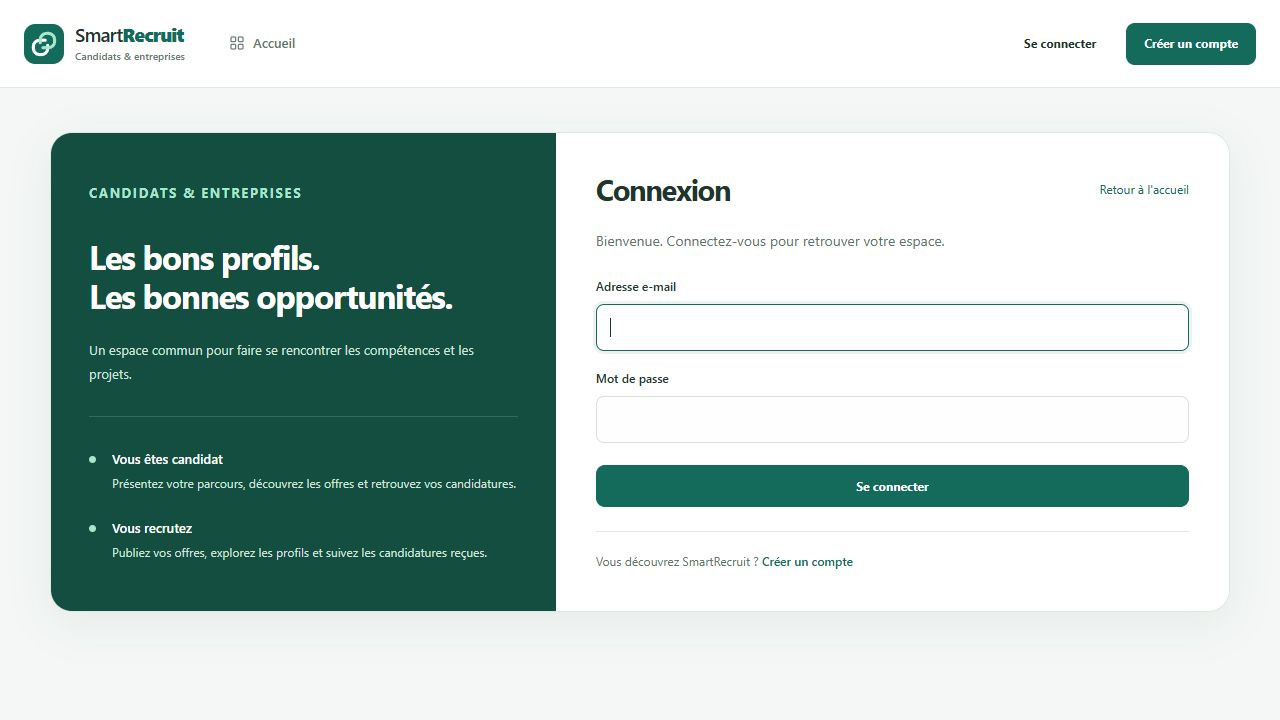
\includegraphics[width=.94\linewidth,height=.74\textwidth,keepaspectratio]{figures/screenshots/01-connexion.png}
\caption{Interface de connexion à SmartRecruit}
\label{fig:interface-01-connexion}\end{figure}
\end{landscape}

\begin{landscape}
\subsection{Choix du profil à l'inscription}
{\small\setstretch{1.05}
L'inscription commence par le choix du type de compte : candidat ou recruteur. Chaque option annonce le parcours associé et prépare le formulaire adapté. Le rôle d'administrateur ne fait pas partie des choix publics.\par}


\begin{figure}[H]\centering
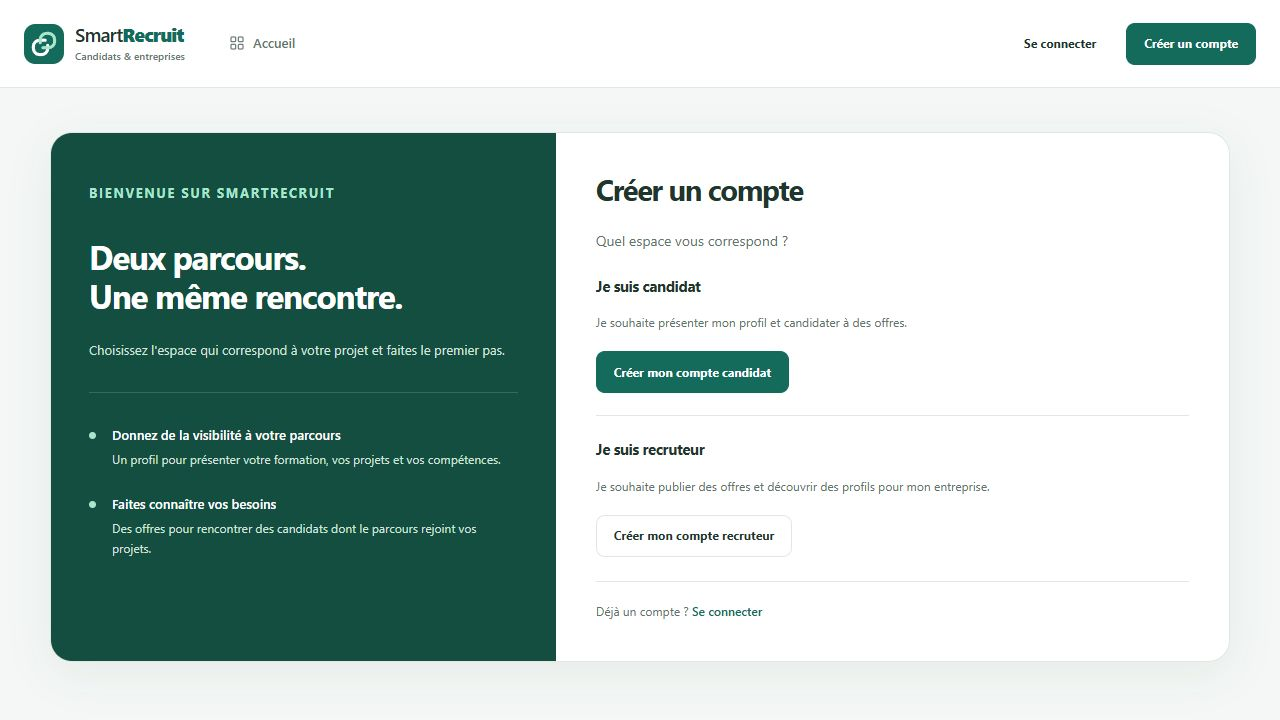
\includegraphics[width=.94\linewidth,height=.74\textwidth,keepaspectratio]{figures/screenshots/02-inscription.png}
\caption{Sélection du type de compte lors de l'inscription}
\label{fig:interface-02-inscription}\end{figure}
\end{landscape}

\begin{landscape}
\subsection{Espace candidat}
{\small\setstretch{1.05}
Le tableau de bord du candidat donne une vue d'ensemble de son profil et de son activité. Les accès aux offres et à la mise à jour du parcours facilitent les actions fréquentes. Le terme candidat employé à l'écran correspond au rôle étudiant du mémoire.\par}


\begin{figure}[H]\centering
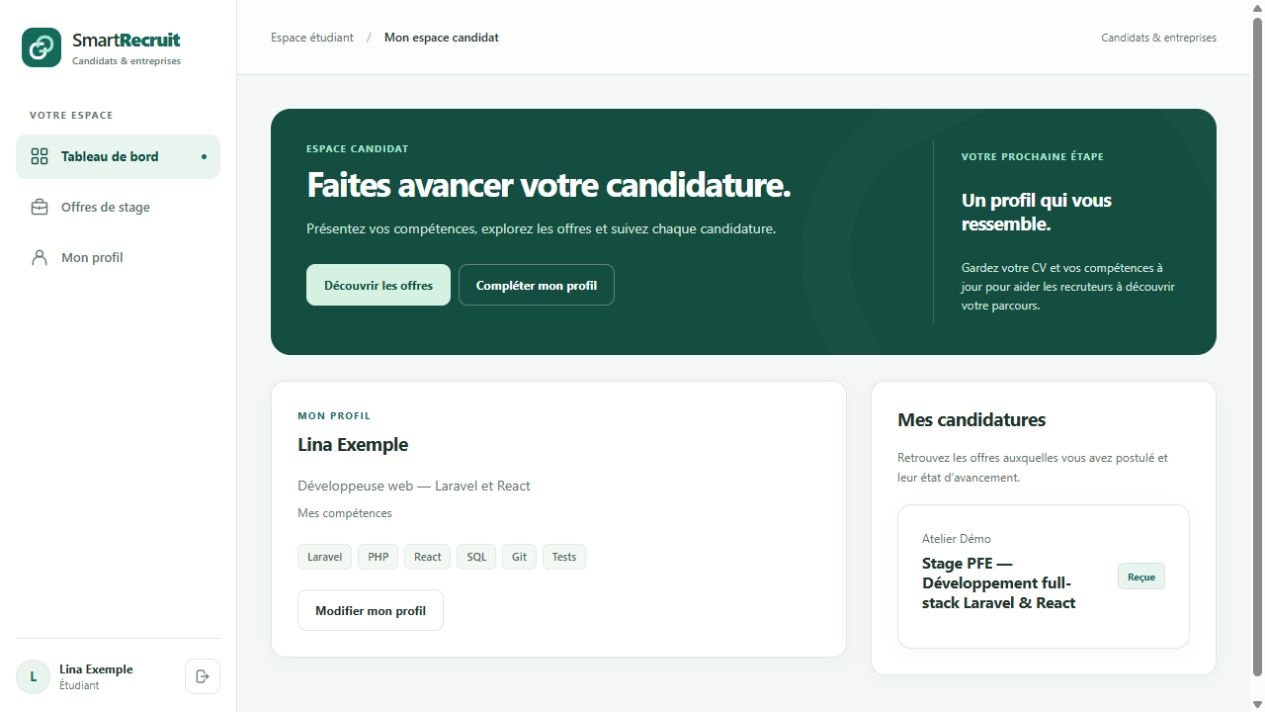
\includegraphics[width=.94\linewidth,height=.74\textwidth,keepaspectratio]{figures/screenshots/05-espace-etudiant.png}
\caption{Tableau de bord du candidat avec données de démonstration}
\label{fig:interface-05-espace-etudiant}\end{figure}
\end{landscape}

\begin{landscape}
\subsection{Profil et informations du CV}
{\small\setstretch{1.05}
La fiche rassemble les informations du parcours, les compétences et les éléments associés au CV. Cette restitution aide à relire les données utilisées lors du rapprochement avec une offre. La possibilité de corriger le profil complète l'extraction automatique décrite par la carte K04.\par}


\begin{figure}[H]\centering
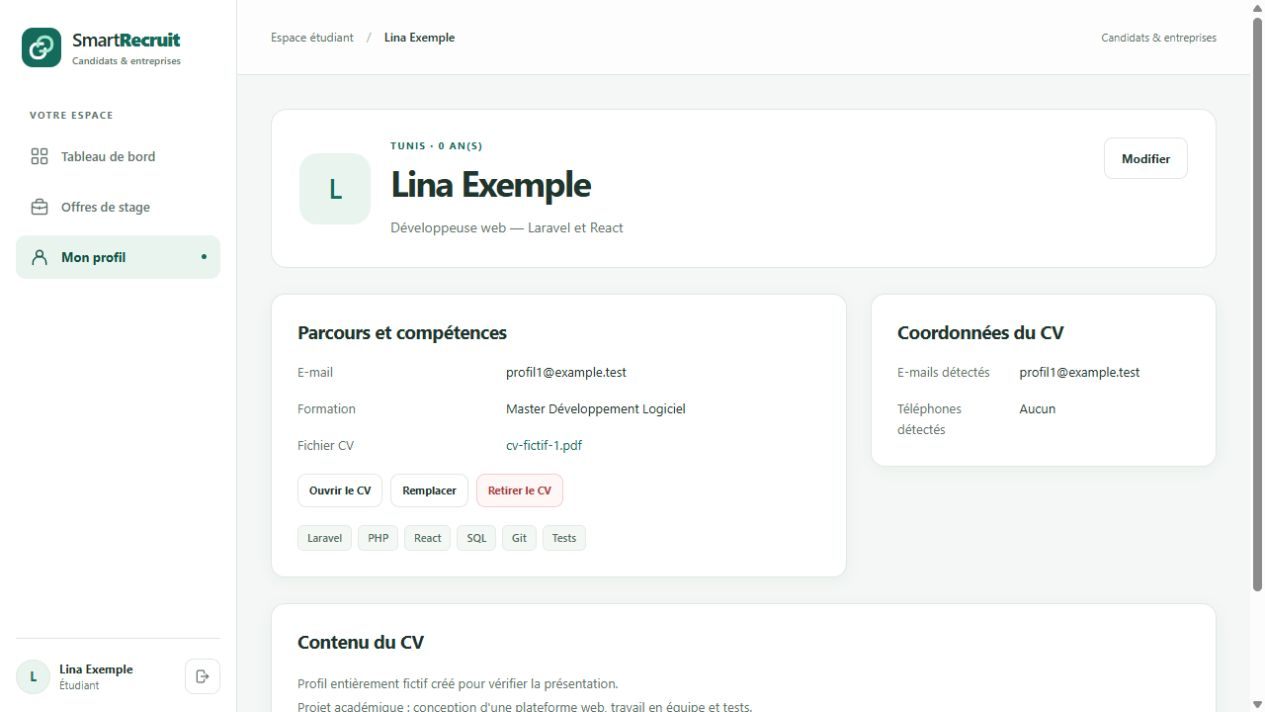
\includegraphics[width=.94\linewidth,height=.74\textwidth,keepaspectratio]{figures/screenshots/09-profil-etudiant.png}
\caption{Présentation du profil candidat et de ses compétences}
\label{fig:interface-09-profil-etudiant}\end{figure}
\end{landscape}

\begin{landscape}
\subsection{Catalogue des offres}
{\small\setstretch{1.05}
Les offres sont présentées avec les informations utiles à leur comparaison et un accès au détail. Des indicateurs de compatibilité et de suivi peuvent accompagner les résultats. Les valeurs visibles ici appartiennent au jeu illustratif ; elles ne mesurent pas la précision du moteur.\par}


\begin{figure}[H]\centering
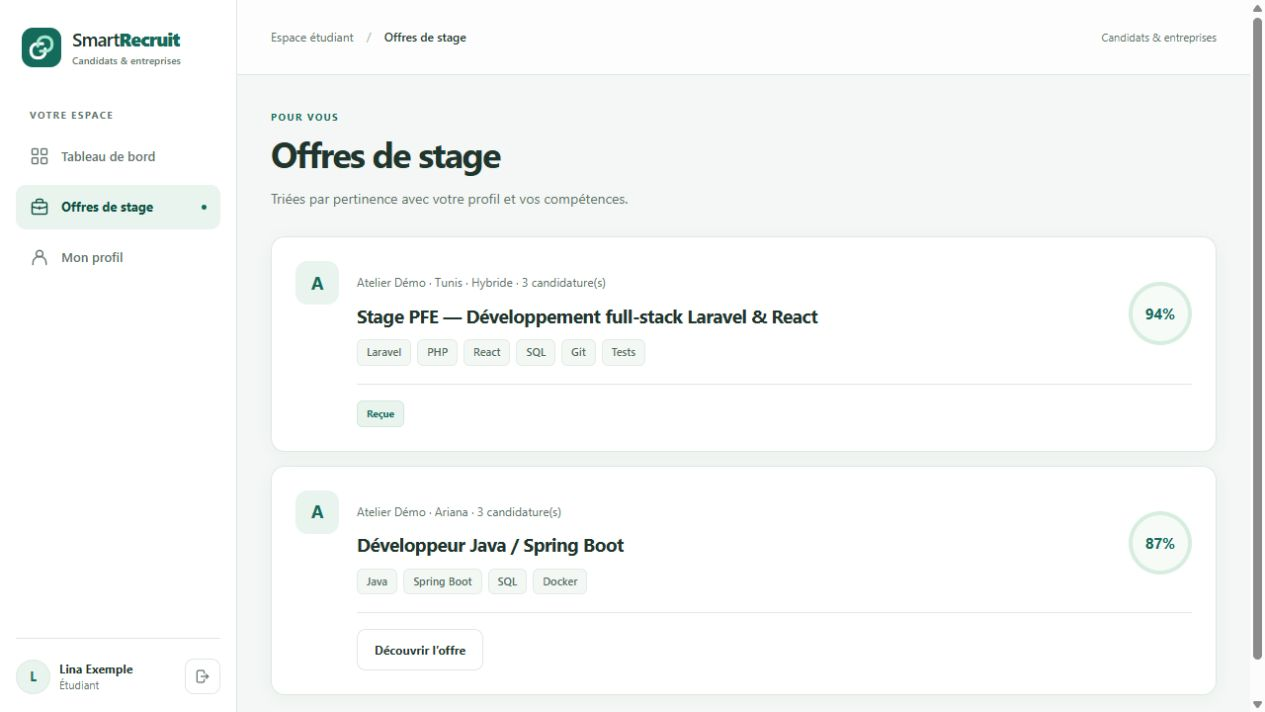
\includegraphics[width=.94\linewidth,height=.74\textwidth,keepaspectratio]{figures/screenshots/06-offres-etudiant.png}
\caption{Catalogue des offres dans l'espace candidat}
\label{fig:interface-06-offres-etudiant}\end{figure}
\end{landscape}

\begin{landscape}
\subsection{Détail d'une offre}
{\small\setstretch{1.05}
La page de détail expose la mission, les exigences et les informations de l'entreprise. Elle replace le rapprochement dans le contexte de l'offre et restitue la situation du candidat lorsqu'une candidature existe déjà. L'utilisateur peut ainsi comprendre le contenu du poste avant de poursuivre son suivi.\par}


\begin{figure}[H]\centering
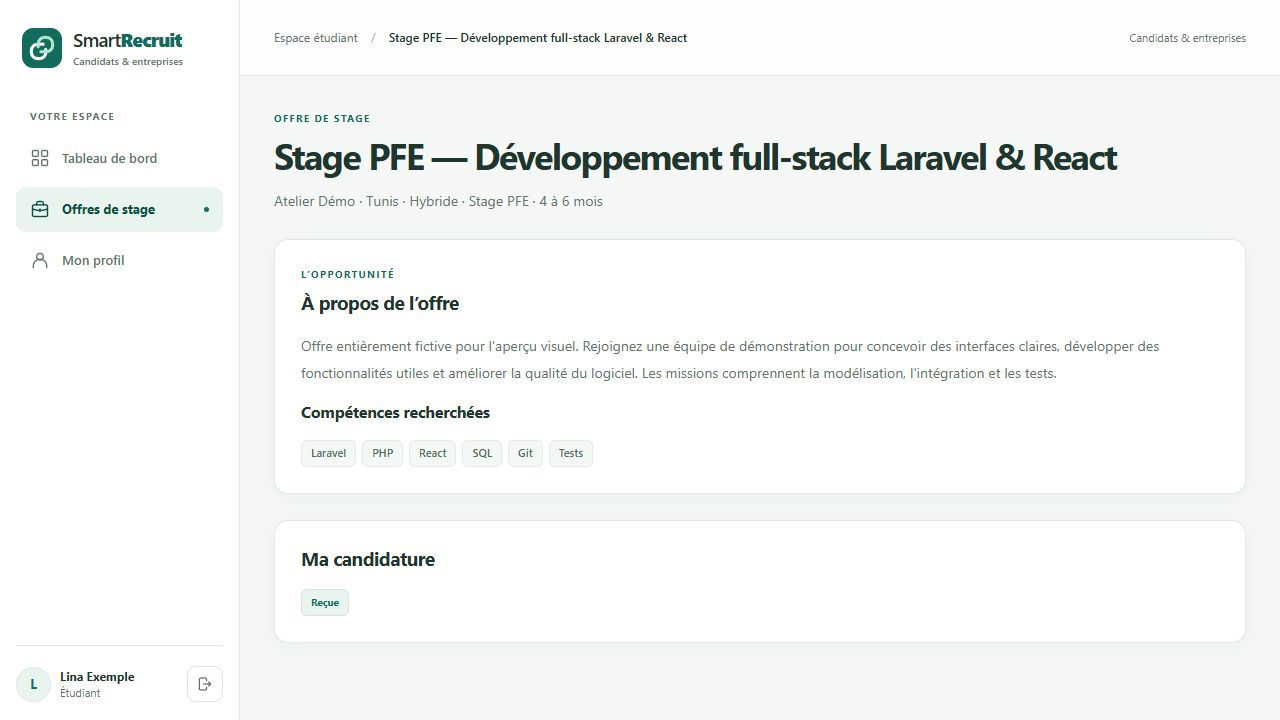
\includegraphics[width=.94\linewidth,height=.74\textwidth,keepaspectratio]{figures/screenshots/07-detail-offre.png}
\caption{Consultation d'une offre et de ses exigences}
\label{fig:interface-07-detail-offre}\end{figure}
\end{landscape}

\begin{landscape}
\subsection{Espace recruteur}
{\small\setstretch{1.05}
Le tableau de bord recruteur synthétise l'activité de ses offres et oriente vers leur gestion. Les filtres et les accès au vivier structurent le travail de consultation. Cette vue met en relation les cartes K05, K08 et K09, consacrées aux offres, aux décisions et au suivi.\par}


\begin{figure}[H]\centering
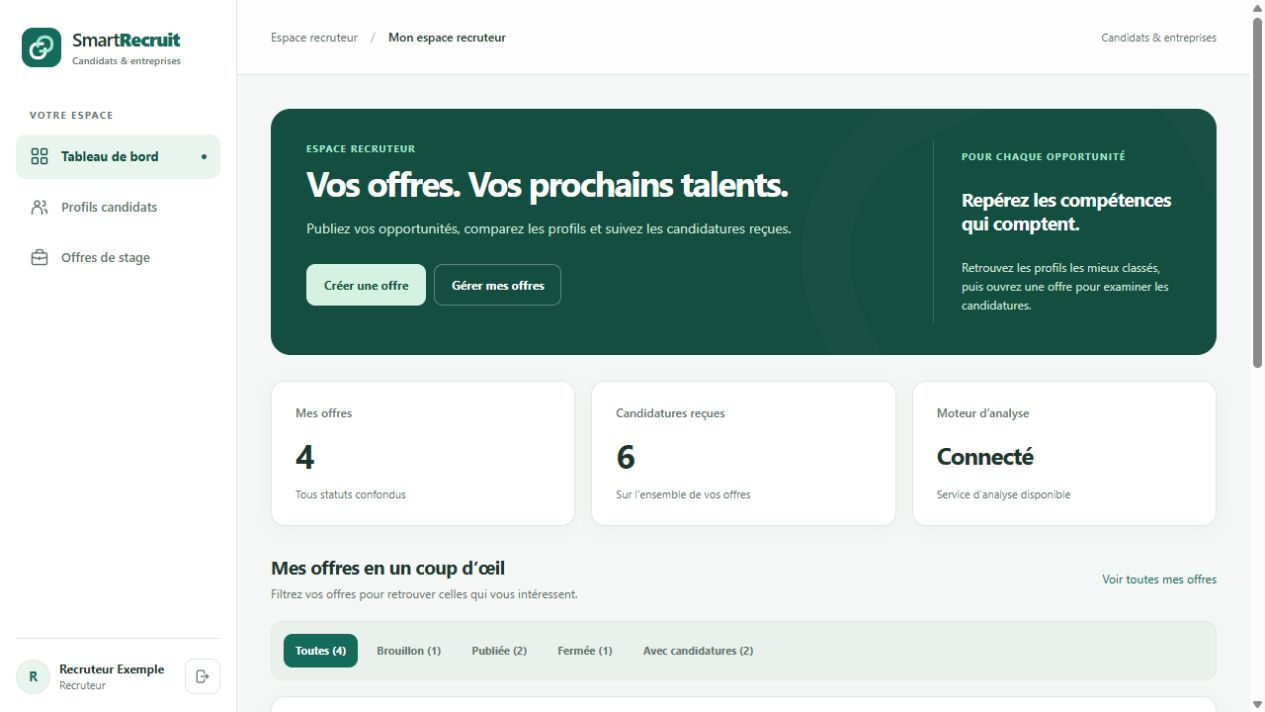
\includegraphics[width=.94\linewidth,height=.74\textwidth,keepaspectratio]{figures/screenshots/04-espace-recruteur.png}
\caption{Tableau de bord du recruteur}
\label{fig:interface-04-espace-recruteur}\end{figure}
\end{landscape}

\begin{landscape}
\subsection{Création d'une offre}
{\small\setstretch{1.05}
Le formulaire permet de décrire une opportunité et les compétences recherchées. La capture montre sa partie supérieure, avec les premiers champs nécessaires à la publication. Les informations saisies alimentent ensuite la consultation de l'offre et sa comparaison avec les profils.\par}


\begin{figure}[H]\centering
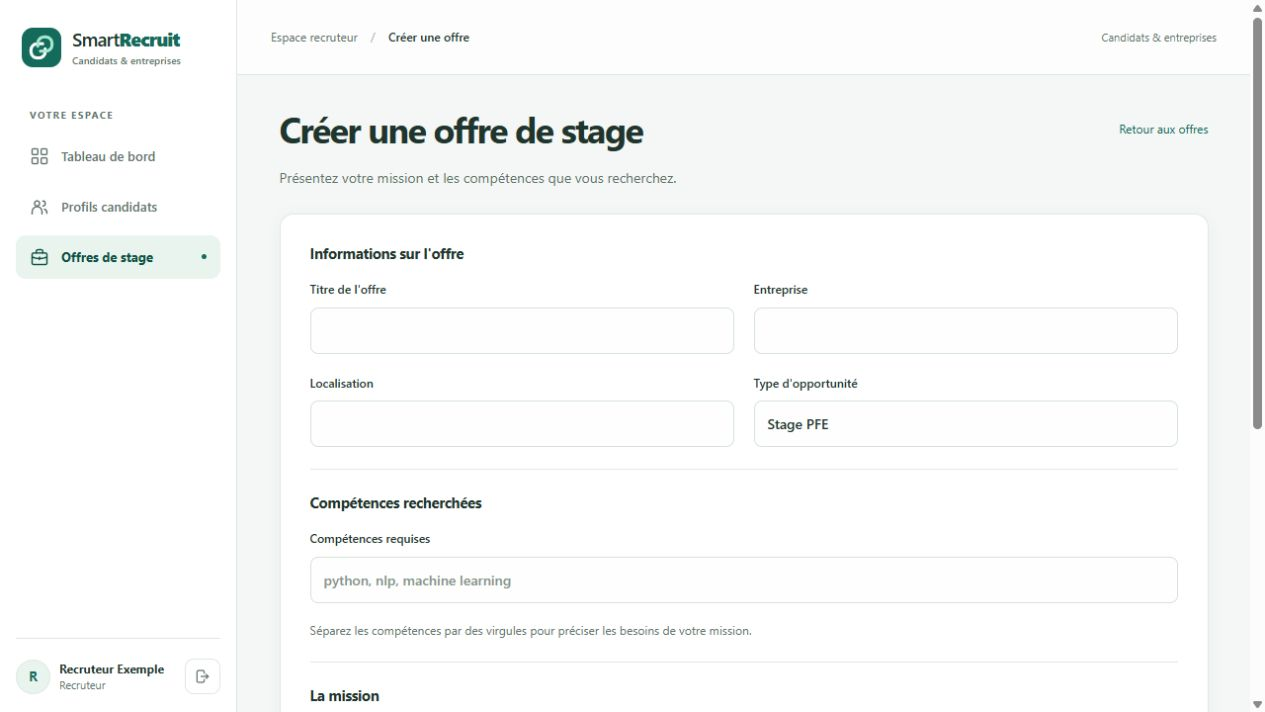
\includegraphics[width=.94\linewidth,height=.74\textwidth,keepaspectratio]{figures/screenshots/10-creation-offre.png}
\caption{Partie supérieure du formulaire de création d'une offre}
\label{fig:interface-10-creation-offre}\end{figure}
\end{landscape}

\begin{landscape}
\subsection{Vivier des candidats}
{\small\setstretch{1.05}
La liste des profils permet au recruteur de parcourir le vivier et d'accéder aux fiches détaillées. Les informations synthétiques facilitent une première lecture des parcours. La présence d'une personne dans ce vivier ne signifie pas qu'elle a postulé à une offre donnée.\par}


\begin{figure}[H]\centering
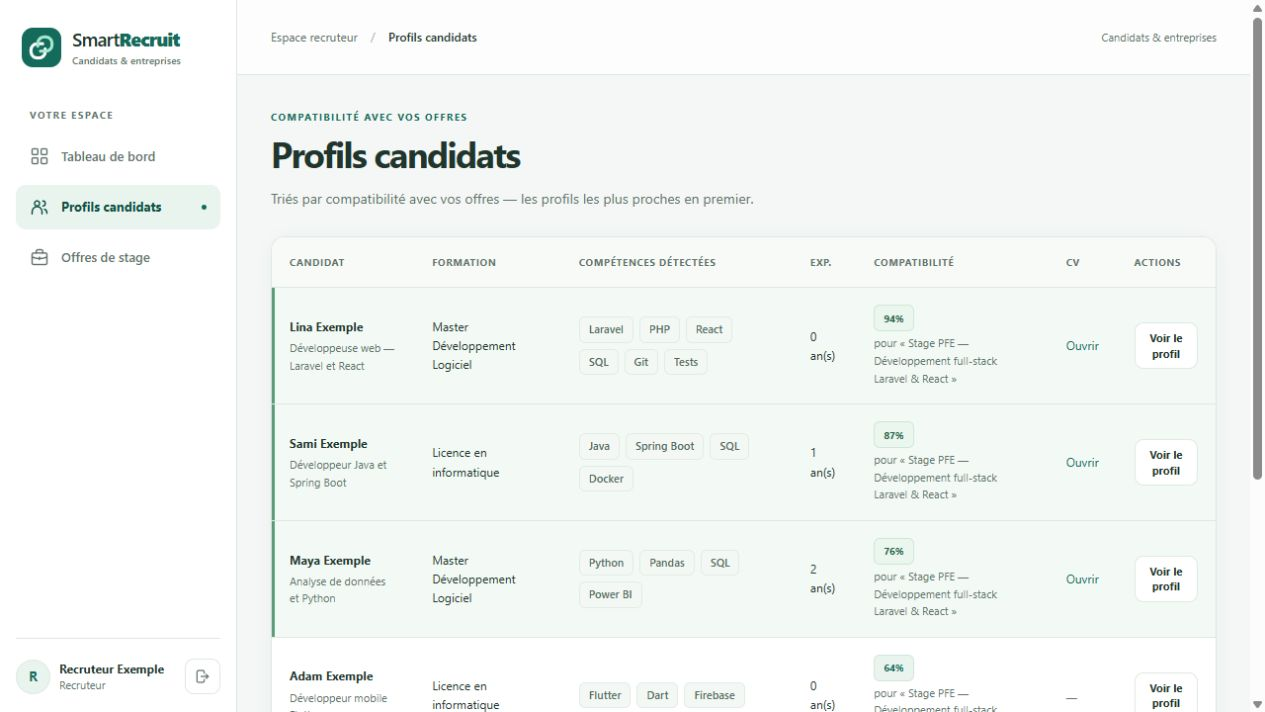
\includegraphics[width=.94\linewidth,height=.74\textwidth,keepaspectratio]{figures/screenshots/12-profils.png}
\caption{Consultation du vivier de profils par le recruteur}
\label{fig:interface-12-profils}\end{figure}
\end{landscape}

\begin{landscape}
\subsection{Classement pour une offre}
{\small\setstretch{1.05}
Le classement associe chaque profil à un score et à des éléments d'explication, notamment les compétences rapprochées ou manquantes. Les actions de décision concernent les candidatures existantes. La capture est centrée sur cette section de la page ; les scores sont des valeurs de démonstration.\par}


\begin{figure}[H]\centering
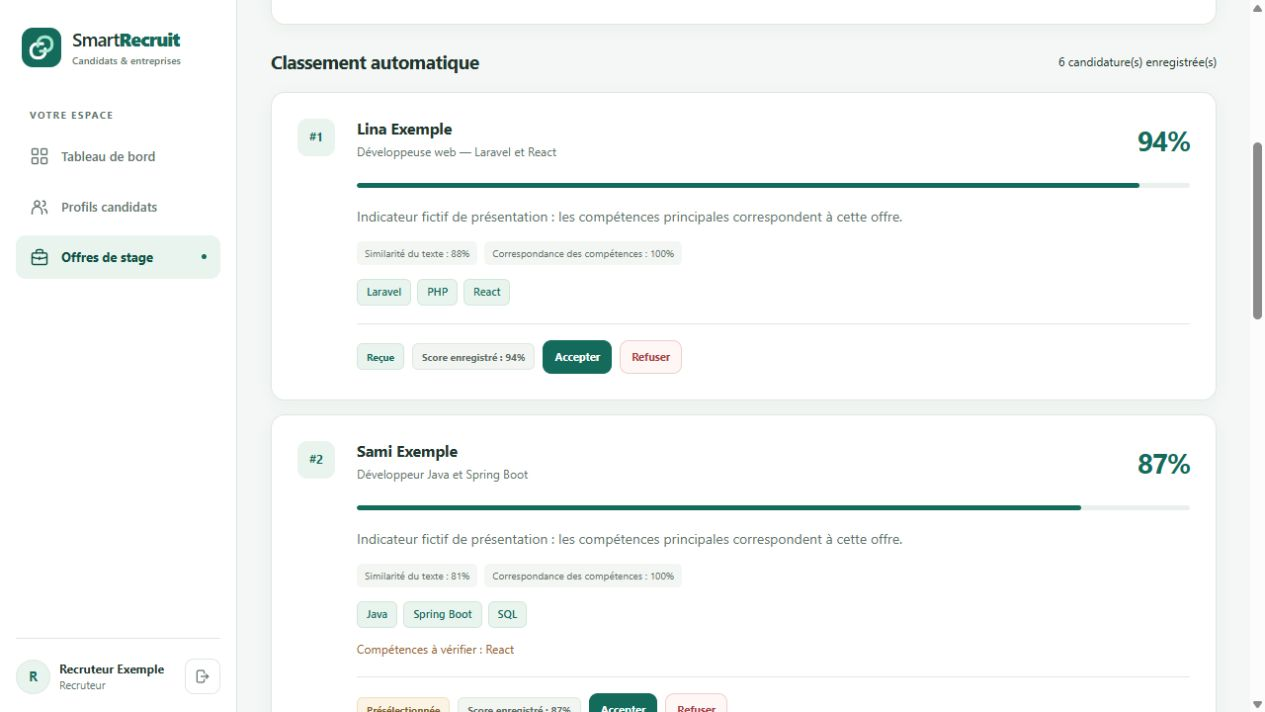
\includegraphics[width=.94\linewidth,height=.74\textwidth,keepaspectratio]{figures/screenshots/08-classement.png}
\caption{Section de classement des profils pour une offre}
\label{fig:interface-08-classement}\end{figure}
\end{landscape}

\begin{landscape}
\subsection{Supervision administrative}
{\small\setstretch{1.05}
L'espace administrateur fournit une vue transversale des comptes, des offres et des candidatures. Ses accès regroupent les fonctions de supervision et de gestion qui dépassent le périmètre d'un recruteur. Cette séparation rend visibles les responsabilités propres au troisième acteur UML.\par}


\begin{figure}[H]\centering
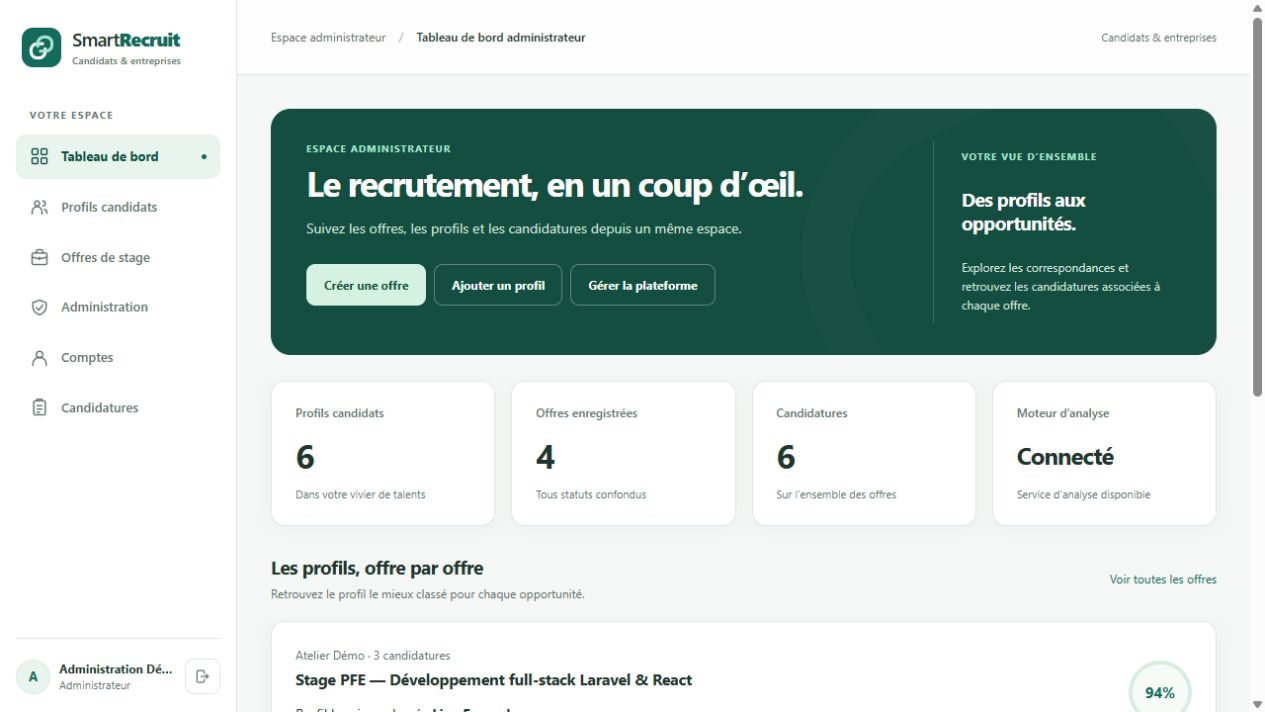
\includegraphics[width=.94\linewidth,height=.74\textwidth,keepaspectratio]{figures/screenshots/03-espace-administrateur.png}
\caption{Tableau de bord de l'administrateur}
\label{fig:interface-03-espace-administrateur}\end{figure}
\end{landscape}

\begin{landscape}
\subsection{Gestion des candidatures}
{\small\setstretch{1.05}
La liste administrative rassemble les candidatures, leur statut et les opérations de gestion. Les filtres permettent de retrouver les éléments actifs ou supprimés logiquement. Le statut métier et la présence dans la corbeille sont deux informations distinctes, conformément au diagramme d'états.\par}


\begin{figure}[H]\centering
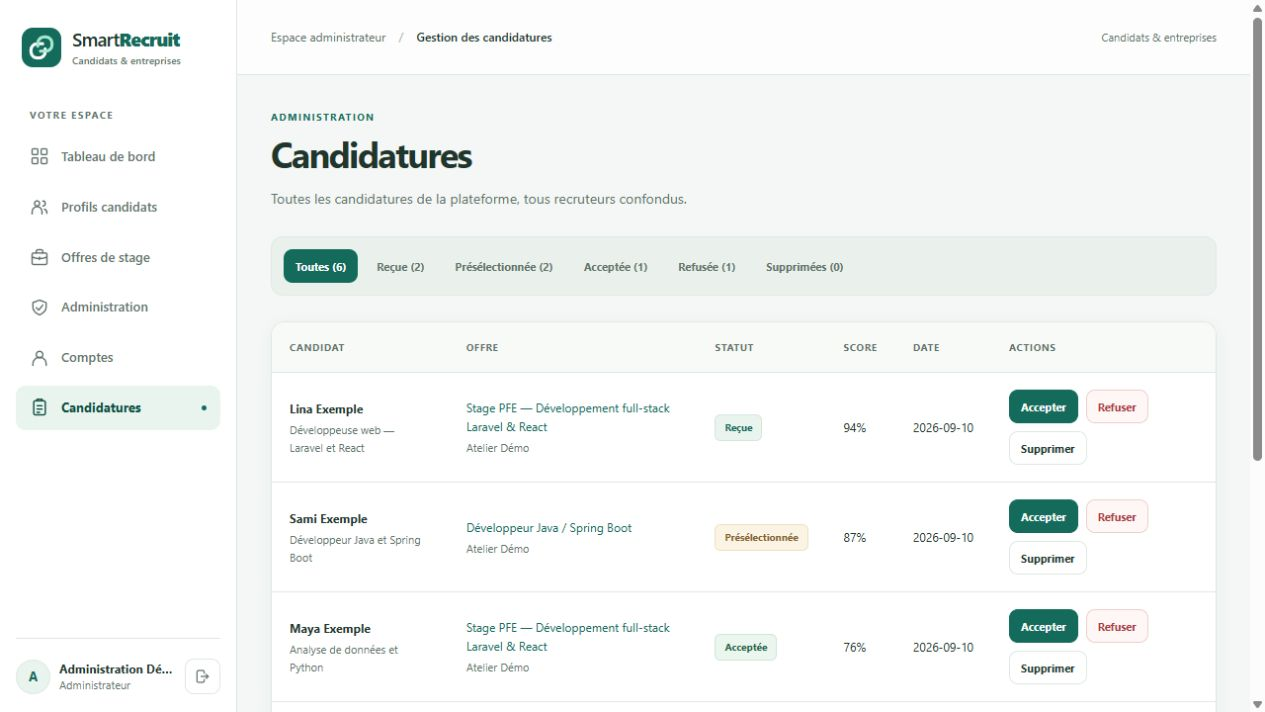
\includegraphics[width=.94\linewidth,height=.74\textwidth,keepaspectratio]{figures/screenshots/11-candidatures.png}
\caption{Suivi et gestion administrative des candidatures}
\label{fig:interface-11-candidatures}\end{figure}
\end{landscape}



\section{Intégration, limites et préparation du déploiement}
Le magasin actif est MySQL. La fonction \code{sr_store} échoue explicitement lorsque la base n'est pas disponible. L'ancien magasin JSON reste un artefact du dépôt et un support d'éléments de démonstration, sans être sélectionné comme persistance de substitution par les routes métier actuelles. Une chaîne de diagnostic ancienne ne suffit pas à établir l'existence d'un repli actif.

La séparation entre démonstration et usage réel demande toutefois un contrôle complémentaire : l'appel \code{all()} conserve un chemin d'initialisation ou de synchronisation de données de démonstration. Ce comportement explique pourquoi les captures du mémoire ont été produites sans ouvrir les routes métier contre la base existante. Avant un déploiement, l'initialisation doit devenir une opération explicite et maîtrisée.

Les paramètres de connexion, les secrets, les chemins de stockage et les ports relèvent de l'environnement. La présence de fichiers Docker ou d'un serveur local n'est pas une preuve de qualification d'une installation. La documentation Laravel et celle de Docker fournissent les mécanismes à configurer ; leur application doit ensuite être vérifiée sur un environnement isolé \cite{laravel-deployment,docker-compose}. Les fichiers CV nécessitent notamment une politique de conservation, des droits adaptés et un accès contrôlé.

La réalisation fournit ainsi une chaîne utilisateur cohérente, de la constitution du profil au suivi d'une candidature. Les captures rendent visibles les choix de présentation ; les contrats et le code expliquent leur fonctionnement. Le chapitre de validation précise la portée des preuves disponibles et les travaux à inscrire dans la réserve Kanban pour consolider cette base.
